\documentclass[a4paper]{jpconf}
\usepackage{graphicx}
\begin{document}
\title{PyFAI, a versatile library for azimuthal regrouping}

\author{J\'er\^ome Kieffer, Dimitrios Karkoulis}

\address{European Synchrotron Radiation Facility; 6 rue Jules Horowitz;
38043 Grenoble; France}

\ead{jerome.kieffer@esrf.fr}

\begin{abstract}
$2D$ area detectors like \textsc{ccd} or pixel detectors have become popular
in 15 last years for diffraction experiments (both in \textsc{waxs},
\textsc{saxs}, single crystal and powder diffraction).
These detectors have a large sensitive area, have high spatial
resolution and provide millions of pixels. PyFAI was designed to reduce \textsc{saxs} and
\textsc{waxs} images taken with those detectors into $1D$ curves (azimuthal
integration) or $2D$ images (a radial transformation named caking), usable by other software
for analysis such as Rietveld refinement.

As a library, the aim of pyFAI is to be integrated into other tools like
PyMca\cite{pymca} or \textsc{edna}\cite{edna} with a clean pythonic interface. But pyFAI
offers also command line tools for batch processing, exporting data in q-space (for \textsc{saxs}) or 2$\theta$ for
(\textsc{waxs}) and a calibration GUI for optimizing the geometry of the setup
using a reference sample's \textit{powder rings}.  PyFAI shares the geometry
of \textsc{spd}\cite{spd} but can directly import geometries determined by
\textsc{fit2d}\cite{fit2d1996}.
PyFAI has been designed to work with any kind of detector and geometry (transmission or reflection) and
relies on FabIO\cite{fabio}, a library able to read more than 20 image
formats produced by detectors from 12 different manufacturers.

During the transformation from cartesian space $(x,y)$ to polar
space $(2\theta, \chi )$, both local and total intensities are conserved
in order to obtain quantitative results. Technical details on how this
integration is implemented and how it was ported to native C-code and parallelized on graphic card are
discussed in this paper.
\end{abstract}

\section{Introduction}

With the advent of hyperspectral experiments like diffraction tomography in the
world of synchrotron radiation, existing tools for azimuthal integration like
\textsc{fit2d}\cite{fit2d1996} and \textsc{spd}\cite{spd} reached their limits with the fast data rate
needed by such experiments. Even when integrated into massively parallel
frameworks like \textsc{edna}\cite{edna}, such stand-alone programs, due to their
monolithic nature, could not keep pace with the data flow of new detectors.
Therefore we decided to create a new implementation of azimuthal integration
which is easier to optimise for specific computer hardware and is designed to
usa modern parallel hardware features if they are available.

\section{Python Fast Azimuthal Integration}
PyFAI is implemented in Python, which is already very popular for synchrotron
radiation data analysis (PyMca\cite{pymca}, PyNX\cite{pynx}, \ldots) and open
source.

\subsection{PyFAI executables}
PyFAI was designed to be used by scientists needing a simple tool for azimuthal
integration. Two command line programs \textit{pyFAI-waxs} and
\textit{pyFAI-saxs} are provided with pyFAI for performing the
integration of one or many images. The \textsc{waxs} version outputs results in
$2\theta /I$  whereas the \textsc{saxs} version outputs $q/I(/\sigma )$.
Options for those programs are parameter files describing the geometry and mask file. They can
also do some  pre-processing like dark-noise subtraction and flat-field correction.

\subsection{A Python library}
PyFAI is first and foremost a library: a tool of the scientific
toolbox built around IPython\cite{ipython} and NumPy\cite{numpy} to
perform data-analysis either interactively or via scripts.
Figure \ref{notebook} shows an interactive session where an integrator is
created, and image loaded and integrated before being plotted.

\begin{figure}[h]
\begin{center}
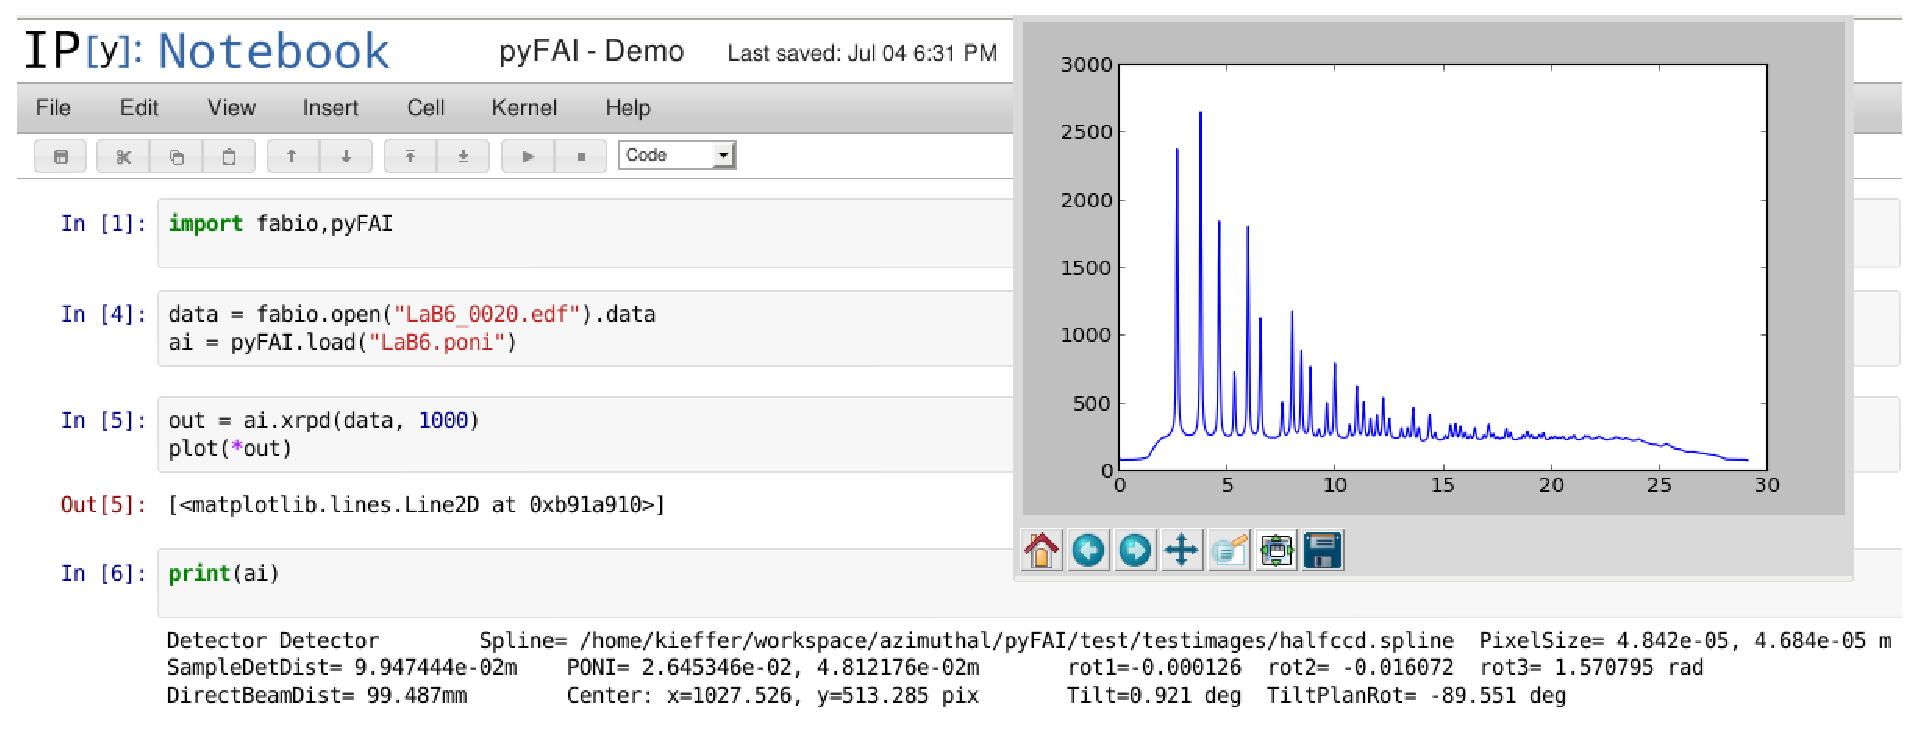
\includegraphics[width=15cm]{img/notebook-l.eps}
\caption{\label{notebook} Example of interactive use of FabIO and pyFAI in the
interactive environment IPython.}
\end{center}
\end{figure}

\section{Regrouping mechanism}
In pyFAI, regrouping is performed using a histogram-like algorithm.
Each pixel of the image is associated to its polar coordinates
$(2\theta , \chi )$ or $(q, \chi )$. Then a pair of histograms of $2\theta$
(or $q$) are built, one non weighted for measuring the number of pixels falling in each bin and
another weighted by pixel intensities.
The division of the weighted histogram by the number of pixels per bin gives
the powder pattern.
$2D$ regrouping (called \textit{caking} in \textsc{fit2d}) is obtained in the
same way using two-dimensional histograms over radial ($2\theta$ or $q$) and azimuthal angles
($\chi$).

\subsection{Pixel splitting algorithm}
Powder diffraction patterns obtained by histogramming have a major weakness where
pixel statistics are low.
%: a high level of  noise is observed close to the beam stop.
A manifestation of this weakness becomes apparent in $2D$-regrouping where most of
the bins close to the beam-stop are not populated by any pixel.
In Figure \ref{rough} many pixels are missing in the low $2\theta$ region,
which is not acceptable.
The  $2D$-regrouping of a smooth image should be smooth(Figure \ref{smooth}).

\begin{figure}[h]
\begin{minipage}{8cm}
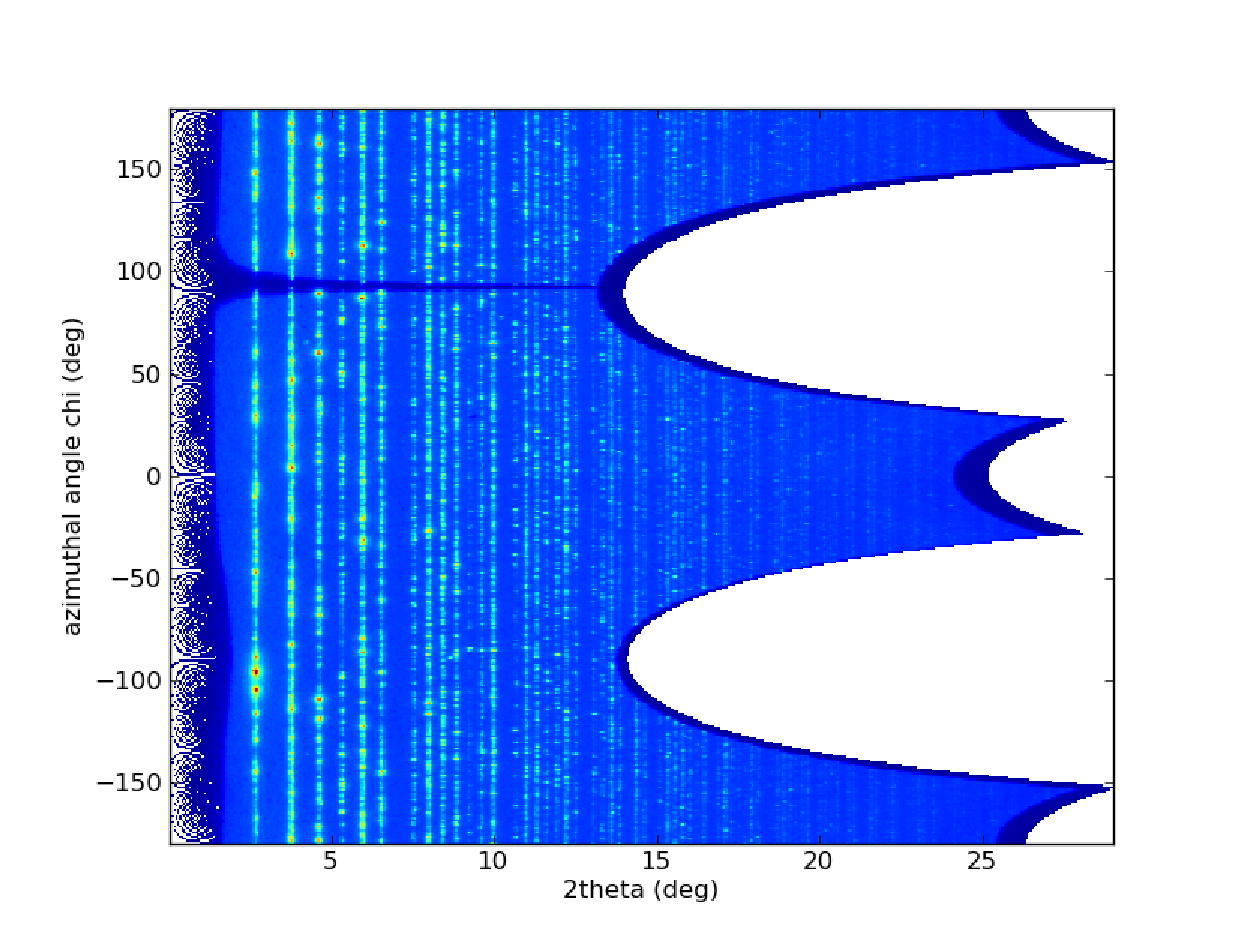
\includegraphics[width=8cm]{img/2Dhistogram.eps}
\caption{\label{rough}$2D$-regrouped image without pixel splitting. Note
the missing pixels near the beam stop and the high-frequency noise patterns.}
\end{minipage}\hspace{5mm}
\begin{minipage}{8cm}
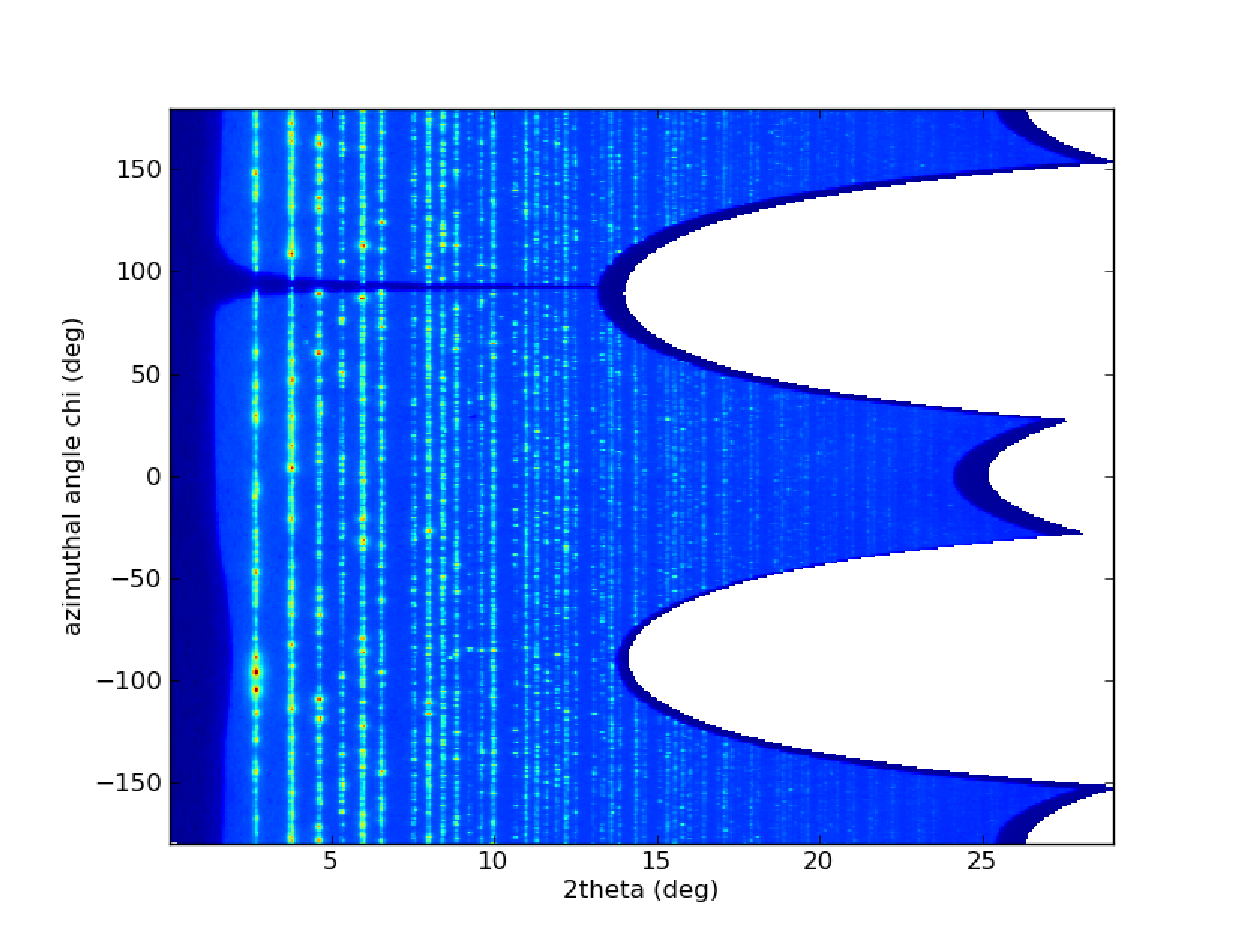
\includegraphics[width=8cm]{img/2DwithSplit.eps}
\caption{\label{smooth}$2D$-regrouped image with pixel splitting. The
transformation of a smooth image remains smooth.}
\end{minipage}
\end{figure}

PyFAI solves this problem by considering, in addition to the pixel's position,
their spatial extension. Each pixel is then split and distributed over the
corresponding bins; intensity being considered as homogeneous within a pixel.

\subsection{Performances and migration to native code}
Originally the regrouping was implemented
using the histogram provided by NumPy\cite{numpy}; then re-implemented in
Cython\cite{cython} with pixel splitting to achieve a four times speed-up.
The computation time is governed by the size of the input image; the performances
are above 30 Mpix/s on a 3.4 GHz Intel corei7-2600.

\subsection{Graphic card implementation}
Graphics Processing Units (\textsc{gpu}s) are composed of hundreds of
arithmetic logic units; they are optimized for highly
parallel algorithms with speed-ups reaching up to 3 orders of magnitude over sequential
code running on Central Processing Units (\textsc{cpu}).
While histograms do not fall into this category, they can nevertheless be
ported to a \textsc{gpu} architecture efficiently.
In order to benefit from \textsc{gpu} acceleration,
the Open Computing Language\cite{opencl} (OpenCL) was used. OpenCL can make use
of multiple different devices such as \textsc{cpu}s and \textsc{gpu}s with very
different features and capabilities.
OpenCL allows the code to work on multiple \textsc{cpu} cores, which was
useful for validation.
As azimuthal integration is a reduction
of millions of pixels into hundreds of bins, double-precision arithmetic is prefered,
which however is not available on all OpenCL devices.
Table \ref{perfs} summarizes the execution time for images coming from
various detectors on a dual-processor computer, either using the
Cython single threaded implementation, either OpenCL on the 16
\textsc{cpu} cores or the 512 \textsc{gpu} cores of the nVidia Tesla C2075 or
GTX580 or 1440 \textsc{gpu} cores of the AMD FirePro v7800 (on the later,
integrations were made in single precision).

\begin{table}[h]
\caption{\label{perfs}Execution time in milliseconds measured on a
Dell T7500 with two Intel Xeon X5690 @3.47GHz and various \textsc{gpu}.}
%: C2075 and GTX580 are professional
%and consumer grade Fermi class nVidia \textsc{gpu} with 512 cores.\\
% The table reports execution time measured in milliseconds for various
% detectors in double precision (except for the AMD FirePro v7800: single precision).}
\vspace{1mm}
\begin{center}
\begin{tabular}{|l|c||c|c||c|c|c|c|}
\hline
Detector type   & Image size 	& \multicolumn{2}{|c||}{\textsc{cpu} X5690}& \multicolumn{4}{|c|}{OpenCL $1D$ regrouping} \\
					& in Mpix		& $1D$	&	$2D$	&	X5690	&	C2075	&	GTX580	&	FirePro* \\
\hline
Pilatus-1M 			& 1  			& 34.4  &	63.1	&	13.9	&	7.2		&	6.3		&	13.8 \\
Half-Frelon 		& 2  			& 76.6  &   132.4   &	23.4	&	14.4	&	12.2	&	18.8 \\
Frelon 				& 4  			& 165.0	&	269.4   &	52.6	&	34.1	&	28.2	&	40.0 \\
Pilatus-6M 			& 6  			& 232.0	&	350.7	&	74.4	&	49.8	&	40.7	&	48.1 \\
Fairchild 			& 16 			& 613.9	&	849.7   &	158.9	&	99.0	&	96.4	&	95.6 \\
\hline
\end{tabular}
\end{center}
\end{table}

The OpenCL implementation of pyFAI is very fast on \textsc{gpu} offering an extra five
times speed-up over the \textsc{cpu} implementation. The profiling of the code revealed new
bottlenecks which will be addressed in future optimizations. The OpenCL
implementation of $2D$ regrouping will also be finalized in a future release.

\section{Conclusion}
The library pyFAI was developed with two main goals:
\begin{itemize}
\item Performing azimuthal integration with a clean programming interface.
\item No compromise on the quality of the result is accepted: a careful
management of the geometry and precise pixel splitting offers total and local intensity
conservation.
\end{itemize}
PyFAI is the first implementation of azimuthal integration on
a graphics card that we are aware of, and the twenty fold speed up observed
opens the door to a new kind of analysis, not even considered before:
a 10-line python script is sufficient for reducing the data of a whole diffraction
tomography experiment, such analysis takes a few minutes using pyFAI on
a 60 x 200 frames dataset when it used to take days.
We believe PyFAI is able to handle the datastreams from the next generation high-speed detectors.

\subsection*{Acknowledgments}
The authors would like to extend their most sincere appreciation to their
colleagues and especially Manuel S\'anchez del R\'io for suggesting
the usage of weighted histograms; Peter B\"osecke for the geometry setup;
V. Armando Sol\'e for his expertise on developing native code under windows and
Jonathan Wright for precise specifications and validations. Porting
pyFAI to \textsc{gpu} would have not been possible without the financial
support of LinkSCEEM-2 (RI-261600).

\subsection*{Appendices}
PyFAI is an open source software released under the GPL licence.
As of July 2012, pyFAI version 0.6, which includes OpenCL
acceleration, is available on the EPN-Campus forge\cite{forge}.
PyFAI depends on Python v2.6 or v2.7, NumPy\cite{numpy} and OpenCL\cite{opencl}.
In order to be able to read images from various detectors, pyFAI relies on the
FabIO\cite{fabio} library available from SourceForge.  
In addition, the graphical user interface for calibration of diffraction setup
uses matplotlib\cite{matplotlib}, SciPy\cite{scipy}, and FFTw3\cite{fftw}.
C, C++ compilers and Cython\cite{cython} are needed to build pyFAI from
sources.
PyFAI is packaged and available in common Linux distributions like Debian
7.0 and Ubuntu 12.04. Installer packages for Windows are also
available on the EPN-Campus forge.

\section*{References}
\bibliographystyle{iopart-num}
\bibliography{biblio}
\end{document}
